%================================================================================
%       Safety Critical Systems Club - Data Safety Initiative Working Group
%================================================================================
%                       DDDD    SSSS  IIIII  W   W   GGGG
%                       D   D  S        I    W   W  G   
%                       D   D   SSS     I    W W W  G  GG
%                       D   D      S    I    WW WW  G   G
%                       DDDD   SSSS   IIIII  W   W   GGG
%================================================================================
%               Data Safety Guidance Document - LaTeX Source File
%================================================================================
%
% Description:
%   Appendix regarding Dark and Dazzle Data
%
%================================================================================
\section{Dark Data and Dazzle Data (Informative)}%
\label{bkm:darkdazzledata}
%
%\dsiwgSectionQuote{Common sense tells us that the government's attempts to solve large problems more often create new ones. Common sense also tells us that a top-down, one-size-fits-all plan will not improve the workings of a nationwide health-care system that accounts for one-sixth of our economy}{Sarah Palin}
\dsiwgSectionQuote{\ldots we can be blind to missing data \ldots that can lead us to conclusions and actions that are mistaken, dangerous, or even disastrous.}{David Hand}

\subsection{Introduction}
Dark and Dazzle data may be viewed as two sides of the same coin. In the former data is hidden, whilst in the latter the important \gls{information} is hidden by an abundance of other data.

\subsection{Dark Data}%
\index{Dark Data|textbf}\index{Data!Dark|see{Dark Data}}%
\label{bkm:darkdata}
%
\subsubsection{Introduction to Dark Data}
This appendix outlines some of the safety implications arising from the issues identified by Prof. David Hand in his work on ``Dark Data'' presented in his book: ``Dark Data: Why What You Don't Know Matters'' \cite{citation:darkdata:hand} and website \cite{citation:darkdata:website}. Dark Data relates to data that is not available, but nevertheless is important, and indeed, in some cases, more important than the data that is available.

Unintentionally Donald Rumsfeld\index{Rumsfeld, Donald} popularised the concept of Dark Data with his famous speech:

\begin{quote}
\dsiwgTextIT{``…there are known knowns\index{Known Knowns}; there are things we know we know. We also know there are known unknowns\index{Known Unknowns}; that is to say we know there are some things we do not know. But there are also unknown unknowns\index{Unknown Unknowns}—the ones we don't know we don't know…''}
\end{quote}

\autoref{fig:lightanddark} neatly shows the dark varieties\index{Dark Data!Varieties} in grey:

\begin{figure}[htbp]
  \centering
  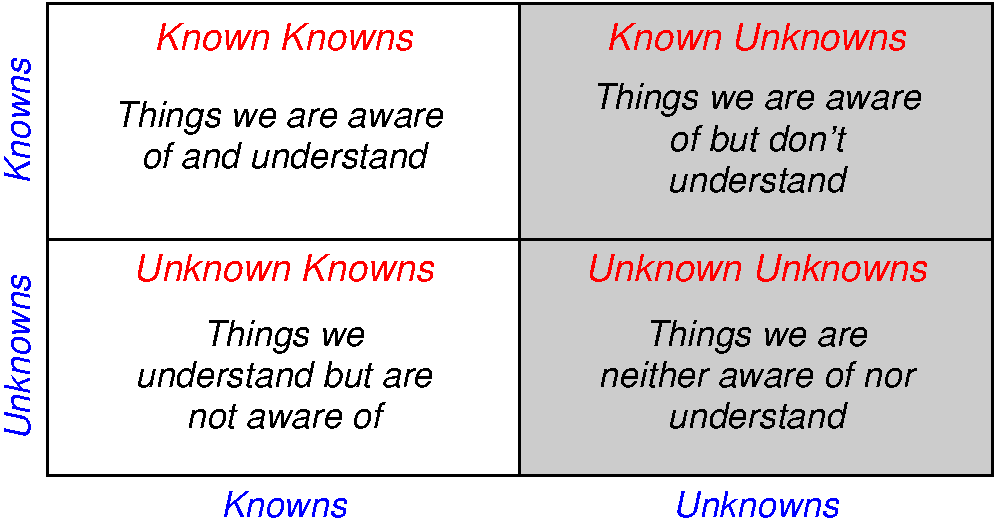
\includegraphics[width=\textwidth/2]{images/darkknowns.pdf}
  %\input{images/darkknowns.latex}
  \caption{Varieties of Dark Data\index{Dark Data!Varieties|textbf}}
  \label{fig:lightanddark}
\end{figure}\index{Unknown Knowns}

\subsubsection{Dark Data Example}
A meeting was held prior to the fatal Challenger disaster in January 1986, to decide whether the flight should go ahead due to the prevailing cold weather and concerns over the performance of O-ring seals at low temperatures. The decision to launch was made on the basis of the following data points that show the temperature at which previous O-ring problems had occurred.

\begin{figure}[htbp]
  \centering
  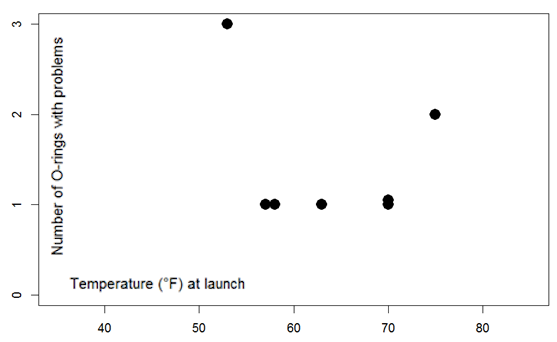
\includegraphics[width=\textwidth/2]{images/darkfailures}
  \caption{O-ring Failures by Temperature}
  \label{fig:o-ringfailures}
\end{figure}

On this basis, it was concluded that: 
``there is nothing irregular in the distribution of O-ring ‘distress’ over the spectrum of joint temperatures at launch between 53 degrees Fahrenheit and 75 degrees Fahrenheit.''
However, there was Dark Data in this dataset --- the data points that show the temperatures for successful launches when there were no O-ring problems were left out. These are shown as the red points in \autoref{fig:o-ringperformance}.

\begin{figure}[htbp]
  \centering
  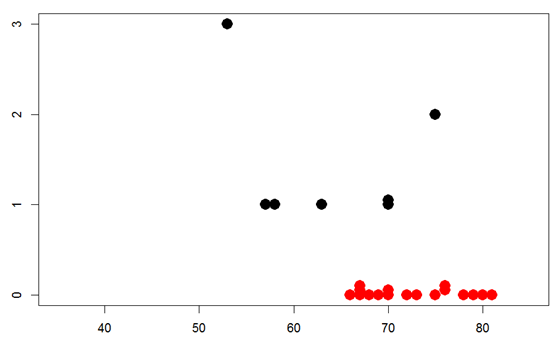
\includegraphics[width=\textwidth/2]{images/darkperformance}
  \caption{O-ring Performance by Temperature}
  \label{fig:o-ringperformance}
\end{figure}

When the Dark Data is included, there is an obvious correlation between temperature and O-ring failures and it is possible the decision to launch may have been different if this additional data had been presented.

\subsubsection{Dark Data Varieties\index{Dark Data!Varieties} and Safety Examples}
In his book, David introduces a taxonomy of 15 varieties of Dark Data. This section discuses each of these from a data safety perspective.

\paragraph{Data We Know Are Missing: ``Known unknowns''}\index{Dark Data!Data We Know are Missing}\label{bkm:dark1}

This case is very common in safety justifications\index{Justification, Safety} where assurance \gls{information} may be withheld for commercial reasons or does not exist, but we know, or are informed, that it isn’t available. Common examples include:
\begin{itemize}
  \item Assurance \gls{information} for \gls{cots}\index{COTS} components is unavailable
  \item \Gls{information} about legacy systems was never produced or is now lost
  \item \Gls{ml} training data restricted to a particular context of use
\end{itemize}
    If this is the case, it can be mitigated\index{Mitigation} in several ways, including use of warnings, training, restrictions of use, etc. Evidence can also be substituted with other more indirect assurance e.g.\ established organisational track-record in the sector, or audit reports.
    
\paragraph{Data We Don’t Know Are Missing: ``Unknown unknowns''}\index{Dark Data!Data We Don't Know are Missing|textbf}\index{Unknown Unknowns}\label{bkm:dark2}
This is the most serious and far-reaching case. Occurrence is hopefully less common than case~\ref{bkm:dark1}, but it is important to acknowledge that it does happen. Some examples are:
\begin{itemize}
  \item The recent Covid-19 Track and Trace data loss (\autoref{bkm:incacc:covidexcel}), where the organisation handling the data was unaware that rows were missing from a spreadsheet for some time is illustrated in \autoref {fig:darknewcases}
  \item Somebody knows a problem with a system but does not tell
  \item Machine learning training data\index{Machine Learning Data} missing edge / corner cases
  \item Key \index{Safety Requirement}safety requirements missed
  \item Change of use never anticipated
  \item Data loss which may be discovered after some period (or indeed never) 
  \item Test cases never thought of, so never created or executed
\end{itemize}

\begin{figure}[htbp]
  \centering
  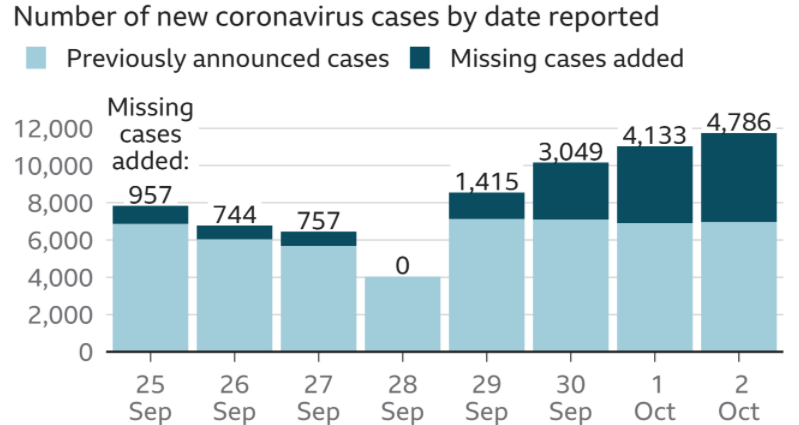
\includegraphics[width=\textwidth/2]{images/darknewcases}
  \caption{Covid-19 Track and Trace Data Loss}
  \label{fig:darknewcases}
\end{figure}

In many cases the loss may be discovered after some time, and it is incumbent on the organisation involved to analyse the impact of the missing data over the time period, including subsequent decisions and actions. Its effects should not be underestimated. This case can fundamentally change the safety picture and is probably in the highest safety risk category.

Data that was missing can subsequently be found. The following options show possible approaches to handling this “rediscovered data”:
\begin{enumerate}[label=\color{dsiwgAccentColour}\roman*)]
  \item Apply the missing data
  \item Ignore the missing data 
  \item Mention that the data was missing but not take it into account, and 
  \item Perform an impact analysis on the missing data and then act according to the results
\end{enumerate}

\paragraph{Choosing Just Some Cases}\index{Dark Data!Choosing Just Some Cases}\label{bkm:dark3}
This is where something or somebody has been selective. Examples might be:
\begin{itemize}
\item Selection of test runs that succeeded (ignoring failed runs and their diagnostics) 
  \item Selective sampling from sensors, or where the sampling intervals are chosen badly
  \item Incorrect filtering of the data, leaving out more cases than intended
  \item Using data from completed forms, finished tasks or only including data which,
    intentionally or not, meets some criteria which excludes the important data.
    This can lead to "Survivorship Bias",
    [Wikipedia ref:
      \href{https://en.wikipedia.org/wiki/Survivorship\_bias}
           {https://en.wikipedia.org/wiki/Survivorship\_bias}]
    of which the following article has a good example from WW2 aircraft where examining the bullet
    holes on aircraft returning from missions could have led to the wrong conclusion:
    \href{https://www.dgsiegel.net/talks/the-bullet-hole-misconception}
         {https://www.dgsiegel.net/talks/the-bullet-hole-misconception}
\end{itemize}
Note that with complex or informal criteria the effects could be as case~\ref{bkm:dark2}, i.e.\ you don’t know what has been left out.

Mitigations\index{Mitigation} include use of peer review, independent teams, and audits. It is important to ask questions and challenge the data selected to be sure it can be justified.

\paragraph{Self-Selection}\index{Dark Data!Self-selection}\label{bkm:dark4}
This is considered to be similar to case~\ref{bkm:dark3}, but could be even more informal or ambiguous. Again mitigations\index{Mitigation} include: use of peer review, independent teams, and audits.

\paragraph{Missing What Matters}\index{Dark Data!Missing What Matters|textbf}\label{bkm:dark5}
This was considered similar to case~\ref{bkm:dark2} in impact terms, and might well be considered the “Elephant in the Room”. Examples might be:
\begin{itemize}
\item Measuring the wrong things, e.g.\ poor safety metrics / indicators
  \item Too much data to deal with or analyse, so some is ignored
  \item Too much filtering or processing, so losing \gls{information} along the way
  \item Being too close to the data, i.e.\ the “wood for the trees”. This is when the detail masks the overall issue with data, e.g.\ a slow trend or bias masked by peaks.
\end{itemize}

Mitigations\index{Mitigation} include independence as~\ref{bkm:dark3} and~\ref{bkm:dark4} but also “taking a step back” to look at the bigger picture.

\paragraph{Data Which Might Have Been}\index{Dark Data!Data Which Might Have Been}\label{bkm:dark6}
This is where it is impossible to obtain the relevant data as a consequence of how the system/scenario is constructed. This was considered an interesting and important case.

This could for example, be due to an inappropriate system architecture e.g.\ single data channel when a multiple channel approach should have been used, such as in the \index{Boeing 737}Boeing 737 MAX~8 accidents (see section H.2). It is therefore important that Mitigations\index{Mitigation} are in place at design time, as they are often very difficult to retro-fit.

Mitigations\index{Mitigation} include assessing the data collection opportunities gained or lost from the design or architectural approach --- at design time.

\paragraph{Changes with Time}\index{Dark Data!Changes With Time}\label{bkm:dark7}
This is a common problem in a safety context. Data in safety systems often becomes obsolete or out of date and may still be mistakenly used. Some examples are:
\begin{itemize}
\item System \gls{configuration data} not kept up to date as software\index{Software Changes} or hardware changes
  \item Medical drug interaction \glspl{database}
  \item Software patches requiring updates to configuration or system data, which is not always done
\end{itemize}

Mitigations\index{Mitigation} include keeping \gls{critical data} up to date and regularly refreshed, and knowing how old the data is in the first place.

\paragraph{Definitions of Data}\index{Dark Data!Definitions of Data}\label{bkm:dark8}
This was considered a common case for systems with \glspl{database} or those exchanging data with external systems, e.g.
\begin{itemize}
\item Taxonomies e.g.\ in machine learning categorisation schemes
  \item Data schemas in medical record systems 
  \item Interface specifications\index{Interface!Specification} and data definitions\index{Data!Definition}, which often evolve over time. These can render old data obsolete / subject to misinterpretation, and often needing migration/translation or re-interpretation.
\end{itemize}

Mitigations\index{Mitigation} include keeping a list of known changes / incompatibilities and documenting the changes or fixes that have to be applied to make the data usable or consistent.

\paragraph{Summaries of Data}\index{Dark Data!Summaries of Data}\label{bkm:dark9}
This is often seen in data about safety systems and projects:
\begin{itemize}
\item Safety metrics or indicators where data is aggregated to create a composite value
  \item Data fusion across multiple sensors
Summaries can be misleading or cause “boundary reactions”, e.g. Red-Amber boundary.
\end{itemize}

Mitigations\index{Mitigation} include thinking about what missing data could cause (i.e.\ performing sensitivity analysis) --- for instance, what decisions might be made erroneously due to certain data values being omitted, late or slightly perturbed.

\paragraph{Measurement Error and Uncertainty}\index{Dark Data!Measurement Error and Uncertainty}\label{bkm:dark10}
Sensors can degrade and fail over time, especially in harsh environments such as automotive, marine or aviation:
\begin{itemize}
\item Sensors may feed faulty or biased data into systems
  \item Sampling techniques can cause some artefacts in themselves
  \item Interval polling interval can lead to misleading readings
  \item Data fusion can be impacted if multiple sensor values are combined
\end{itemize}

Hence sensors need to be regularly maintained and calibrated or replaced, and their interfaces\index{Interface!Sensor} need to be able to detect any problems and report faults. 

\paragraph{Feedback and Gaming}\index{Dark Data!Feedback and Gaming}\label{bkm:dark11}
This can often happen in safety justifications\index{Justification!Safety} or test case production:
\begin{itemize}
\item Early production of a safety argument could lead to only those artefacts that support the claim being generated, e.g.\ requirements-based testing vs.\ stress testing
  \item Confirmation bias in safety justifications\index{Justification, Safety} and can cause over-optimism
\end{itemize}

Mitigations\index{Mitigation} include the use of dialectic argument approaches (where both positive and negative cases can be considered). It is also useful to get a second opinion, independent review or a ‘fresh pair of eyes’ to check the justification.

\paragraph{\glsfmttext{information} Asymmetry}\index{Dark Data!Information Asymmetry}\label{bkm:dark12}
This is common where there are multiple stores or sources of the same data:
\begin{itemize}
\item Multiple / backup \glspl{database} where they are not kept in sync
  \item Image recognition systems that learn, but fail to share data
  \item Issues of divergence of data across multiple sources.
\end{itemize}

Comparisons, reviews and data audits may help in these cases. In general the issue of divergence across multiple data sources needs to be recognised and addressed in the most appropriate technical, and ideally automated, way.

\paragraph{Intentionally Darkened Data}\index{Dark Data!Intentionally Darkened Data}\label{bkm:dark13}
This can and does happen, e.g.
\begin{itemize}
\item Defence, security and government sectors where data is purposefully hidden or destroyed
  \item Records intentionally deleted after an accident to cover up what really happened
\end{itemize}

This can be mitigated\index{Mitigation} using appropriate technical measures (e.g.\ blockchain, digital signatures, off-site backups), and also robust procedures with oversight.

\paragraph{Fabricated and Synthetic Data}\index{Dark Data!Fabricated and Synthetic Data}\label{bkm:dark14}
Fabrication (i.e.\ making up the data) is surprisingly common, e.g.\ in medical, policing and maritime sectors. Sometimes it is created with the best of intentions as it was not produced or collected at the right time and is now required (e.g.\ for an audit), but sometimes it is created to mask a problem. Synthetic data is often used where there are difficulties in producing enough real data with the right characteristics:
\begin{itemize}
\item Data is retrospectively entered / patched to make a “clean” record
  \item Synthetic autonomous vehicle training \glspl{database} can have issues with artificial data if not realistic
\end{itemize}

Possible mitigations\index{Mitigation} include comparisons with current real-world data and checking with historical data.

\paragraph{Extrapolating Beyond Your Data}\index{Dark Data!Extrapolating Beyond Your Data}\label{bkm:dark15}
Systems, especially machine learning systems (see Appendix J) have to cope with values outside of their training data\index{Machine Learning Data}, but the outcomes may be unexpected:
\begin{itemize}
\item Bizarre results from recognition / detection systems may result
\end{itemize}

Mitigations\index{Mitigation} include use of machine learning training data\index{Machine Learning Data} containing edge/corner cases, boundary cases, and testing well beyond normal or acceptable ranges to give insight into the system degradation behaviour.
\subsubsection{Summary of Dark Data}
Dark Data is a very useful way of thinking about problems and solutions. It is important to always think of the bigger picture, considering what \gls{information} is not known:

\begin{itemize}
  \item What might have been left out, intentionally or otherwise?
  \item What might be missing due to the way things are done (or the way those things are being executed)?
  \item Could missing items cause any safety problems?
  \item What is outside of the defined operational domain?
  \item Can you present your results / outputs in a way that shows the dark data?
\end{itemize}

\subsubsection{Further Reading}
A number of resources are available for further \gls{information} on how Dark Data relates to data safety:
\begin{itemize}
\item The October 2020 edition of the SCSC Newsletter \cite{citation:SCSC160} contains articles both by David Hand and on Dark Data Safety.
  \item A presentation on Dark Data given by David Hand to the \gls{dsiwg} \cite{citation:darkdata:presentation1};
  \item A presentation by Mike Parsons given at the University of York \cite{citation:darkdata:presentation2}.
\end{itemize}
%
%
% Start of Dazzle Data section
%
%
\subsection{Dazzle Data}\index{Dazzle Data|textbf}\index{Data!Dazzle|see{Dazzle Data}} \label{bkm:dazzledata}
%
%\dsiwgSectionQuote{A ship in a port is safe, but that's not what ships are built for}{Grace Hopper}

%\dsiwgSectionQuote{Don't fix the blame, fix the problem}{Keith Pennington}

% Quote previously used at head of Dazzle section: 
%\dsiwgSectionQuote{Camouflage is a game we all like to play, but our secrets are as surely revealed by what we want to seem to be as by what we want to conceal}{Russell Lynes}

\subsubsection{Introduction to Dazzle Data}
This appendix outlines some of the safety implications arising from the issues identified by
``Dazzle Data'' in contrast to ``Dark Data''\index{Dark Data} presented in David Hand's book:
``Dark Data: Why What You Don't Know Matters'' \cite{citation:darkdata:hand}
and website \cite{citation:darkdata:website}.
Dark Data\index{Dark Data} relates to data that is not available but nevertheless is important.

``Dazzle Data'' refers to spurious, superfluous or unexpected data that masks and confuses the picture and can reduce your ability to see details, and indeed the whole picture --- a bit like noise or camouflage.

\begin{quote}
  It is data you don't want, didn't ask for, arrives more frequently than expected, is redundant, or data that arrives at an unexpected or inconvenient time or in the wrong format or sequence, so requiring extra resources to deal with\dots
\end{quote}

At first sight it might be thought this is just an annoyance rather than a problem,
however Dazzle Data can mask, distort or prevent usage of the real or desired data.
It can hide the true picture as in ``wood for the trees'' and in the worst case create real problems. 

Some examples of such false positive alerts that cause real alerts to be ignored are:
\begin{itemize}
  \item The classic case of ``Crying Wolf''.
  \item Denial of Service Attack, when servers can be blocked with useless requests that cannot be distinguished from the real requests.
\end{itemize}

Data which is truly spurious and believable (e.g. generated by extensive electrical noise, or fabricated to mask a fraud) may be accepted as valid data, leading to potentially hazardous results. 

Varieties of Dazzle Data may be identified\index{Dazzle Data} in the same grid manner as Dark Data\index{Dark Data}, as shown in \autoref{fig:dazzle}, where the yellow areas indicate potential dazzle data.

\begin{figure}[htbp]
  \centering
  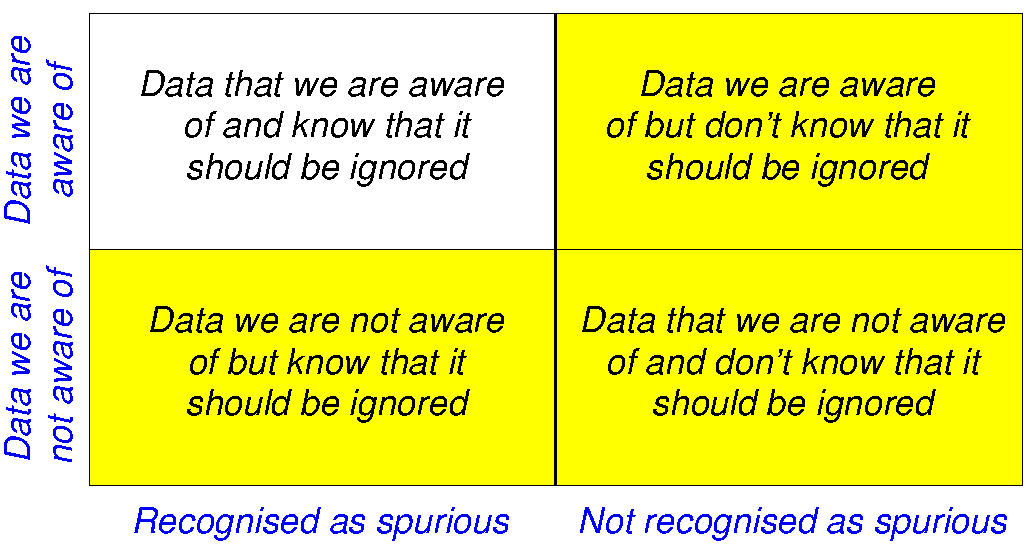
\includegraphics[width=\textwidth/2]{images/dazzleknowns.pdf}
  \caption{Dazzle Data Varieties}
  \label{fig:dazzle}
\end{figure}

\clearpage
\subsubsection{Dazzle Data Examples}

\paragraph{Data We Are Aware Of --- Recognised as Spurious}\index{Dazzle Data!Data We Know are Spurious or Unneeded}
Repeated false positive alerts (e.g. from faulty sensors or alarms). These tend to be annoying irritants rather than safety issues, however they can lead to alarms being permanently switched off, masking true problems. An example from everyday life might be removing the battery from a badly place smoke alarm in a kitchen which repeatedly sounds when the toaster is used.

\paragraph{Data We Are Aware Of --- Not Recognised as Spurious}\index{Dazzle Data!Data We Don't Know are Spurious or Unneeded}
Electromagnetic interference (EMI) affecting transmitted data is a good example of this case; we know it exists as a possibility but don't know how it might affect data in a system or a communications path, and this could be in different ways at different times or days.

\paragraph{Data We Are Not Aware Of --- Recognised as Spurious}\index{Dazzle Data!Data We Know are Spurious or Unneeded}
In many cases we do not know what changes or corruptions may affect the data, but we have strong correction mechanisms to cope with the problems regardless. A good example is data stores on a spacecraft which have redundancy and error correcting codes built-in and so can deal with the majority of corruptions caused by cosmic rays.

\paragraph{Data We Are Not Aware Of --- Not Recognised as Spurious}\index{Dazzle Data!Data We Don't Know are Spurious or Unneeded}
An example of this is where data is mistakenly added to a machine learning training data\index{Machine Learning Data} set resulting in bizarre and possibly hazardous behaviours of the system using it (e.g. an autonomous road vehicle). It is paramount that data used for such image recognition systems filters and excludes potentially dangerous extraneous data arising from unanticipated situations 

\subsubsection{Dazzle Data Varieties\index{Dazzle Data} and Safety Examples}
In his book, David Hand introduces a taxonomy of fifteen varieties of Dark Data\index{Dark Data}. This section discuses each form of Dazzle Data and considers it from a systems and safety assurance perspective.
Some of the varieties are the same as Dark Data\index{Dark Data}, but some are very different.

\paragraph{Data We Know are Superfluous or Unneeded: ``Known Extras''}\index{Dazzle Data!Data We Know are Spurious or Unneeded|textbf}
\label{bkm:dazzledata:case1}

This case is very common in systems where an interface\index{Interface!Flooding} may be flooded with unsolicited messages.
It is also common in  safety justifications\index{Justification, Safety} where assurance \gls{information} may be padded out with extra, irrelevant \gls{information} that can mask the underlying safety argument (which may or may not be intentional).
It can be a serious problem in large, complex safety documents or detailed safety analyses.
Luckily, in this case, the data is recognised as superfluous and can be ignored.
Common examples include:
\begin{itemize}
    \item Mailboxes filled with spam mail, preventing important messages being read
    \item Repeated stall warnings when the aircraft is under control
    \item Assurance \gls{information} in a safety case is included for components which are not part of the solution in use at that site or situation
    \item Assurance \gls{information} about old or legacy components is included but these are now not in service
    \item Machine learning training data\index{Machine Learning Data} contains many cases which are duplicates or very closely related, so adding nothing to the learned behaviour but making the set hard to deal with
\end{itemize}
This case can be mitigated\index{Mitigation} in several ways, including careful filtering, review, use of concise  notations (such as Goal Structuring Notation) to extract the essence, and periodic audits and cleans. 

\paragraph{Data We Don’t Know Are Unneeded or Spurious: ``Unknown Extras''}\index{Dazzle Data!Data We Don't Know are Spurious or Unneeded|textbf}
This is the most serious and far-reaching case, where the additional data is not recognised as unneeded and may be processed, analysed or be left in place when it should be removed. Some examples are:
\begin{itemize}
\item Legacy code in software\index{Software!Legacy} where nobody understands its function, or how it relates to the current code and so is reluctant to remove it. The Ariane 4 Inertial Reference function left in place in the Ariane 501 launch disaster might be such a case. Note that code whose function is known would be under the first case, discussed in \ref{bkm:dazzledata:case1}
    \item Parts of the safety case or safety argument are supplied separately (e.g. by a subcontractor or 3rd party) and they are obscure. In this case it will not be known which parts are relevant to the particular situation. Some \gls{information} may be irrelevant or worse, misleading.
    \item Machine learning training data\index{Machine Learning Data} containing too many outliers, which are not recognised as such
\end{itemize}

In many cases the extra data may be discovered after some time, and it is incumbent on the organisation involved to analyse the impact of the complete set of data which may have been used over the time period, including subsequent decisions and actions. The effect of spurious data should not be underestimated, as it may have masked, prevented or distorted the intended use of the nominal data for some time. This case can fundamentally change the safety picture and is probably in the highest safety risk category.

Data found to be erroneous (i.e. it should not ever have been in the system or in the safety argument) is a problem. The following options show possible approaches to handling this data:
\begin{enumerate}[label=\color{dsiwgAccentColour}\roman*)]
    \item Delete the erroneous data
    \item Accept the erroneous data, i.e. continue using it
    \item Report that the data was erroneous but take no further action 
    \item Establish under what circumstances and situations the erroneous data would have had an effect
    \item Perform a full impact analysis on the effects of the erroneous data and then act according to the results
\end{enumerate}

\paragraph{Data Obscuration: Missing What Matters}\index{Dazzle Data!Data Obscuration}
This is where the meaning of the overall data set becomes obscured due to the extra unnecessary data. Examples might be:
\begin{itemize}
    \item Measuring the wrong things due to excessive noise or too much data to deal with
    \item Processing involving sampling only picks bad data elements
    \item Being too close to the data, i.e. the ``wood for the trees''. This is when the extra data masks the overall issue with the data, e.g. a slow trend or bias hidden by large local variations.
\end{itemize}

Mitigations\index{Mitigation} include review, statistical checks and ``taking a step back'' to look at the bigger picture.
\paragraph{Data Masking in Specific Cases}\index{Dazzle Data!Data Masking in Specific Cases}
This is where the extra data specifically masks, obscures or hides particular data elements (but not all). A particularly nasty case of this is where filters are put in place to remove unwanted data values, but those filters actually remove less (or more) than they should (i.e. don’t remove all unwanted cases or remove valid values as well). Some examples might be:
\begin{itemize}
    \item The number of successful test runs vastly outweighs failed runs and so the failures are not investigated
    \item Incorrect filtering of the data, leaving in some cases that should have been excluded
\end{itemize}

Mitigations\index{Mitigation} include use of review and \index{Completeness!Checks}completeness checks. Note that over-aggressive filtering would create cases of Dark Data\index{Dark Data}.
\paragraph{Masquerade or Fraudulent Data}\index{Dazzle Data!Masquerade or Fraudulent Data}
This is where data has been constructed to fool the system consuming it, hiding, overlaying or replacing the correct data. Often this will be malicious and should be filtered or rejected by the target system, but of course may not be. 
\begin{itemize}
    \item Intentional fraud
    \item Some security attacks
\end{itemize}

Mitigations\index{Mitigation} include audit, blockchain, monitoring, intelligent profiling of data and detection of changes.

\paragraph{Incorrect Definitions of Data}\index{Dazzle Data!Incorrect Definitions of Data}
This is considered a common case for systems exchanging data with external systems, where they may duplicate, translate or incorrectly send multiple messages. They may be time-separated, for instance if communications are lost and then regained, leading to confusion.
\begin{itemize}
    \item Data sent in the wrong rate or units (e.g. every millisecond rather than second)
    \item Data given for the wrong range or duration (e.g. for a month rather than a day
    \item Data sent for the wrong domain or scale (e.g. national values rather than regional)
    \item Text messages re-sent to a mobile phone when coverage restored
\end{itemize}

Mitigations\index{Mitigation} include making sure interface\index{Interface!Specification} specifications are clear and ambiguous, rejecting incorrect size or scale data sets, keeping a list of known changes / incompatibilities and documenting the changes or fixes that have to be applied to make the data usable or consistent.

\paragraph{Summaries of Data}\index{Dazzle Data!Summaries of Data}
Spurious data can affect summaries in a significant way if composite values are calculated, e.g.
\begin{itemize}
    \item Calculations of averages or other statistics affected by duplicates
    \item Spurious outliers can lead to over fitting when analysing data trends
\end{itemize}

Mitigations\index{Mitigation} include audit and assessing what extra data could cause (i.e. performing sensitivity analysis) and establishing what decisions might be made erroneously due to certain data values being present.	

\paragraph{\Glsfmttext{information} Asymmetry}\index{Dazzle Data!Information Asymmetry}
This is common where there are multiple stores or sources of the same data. If one has erroneous duplicate values (i.e. many null values used for padding) then comparisons between them may fail.
\begin{itemize}
    \item Multiple / backup \glspl{database} where they are not kept in sync
    \item Issues of divergence of data across multiple sources.
\end{itemize}

Comparisons, reviews and data audits may help in these cases. In general the issue of divergence across multiple data sources needs to be recognised and addressed in an automated way.

\paragraph{Intentionally Dazzled Data}\index{Dazzle Data!Intentionally Dazzled Data}
This might happen in a secure context where key data is effectively ``camouflaged'' by hiding within large \glspl{item data} (e.g. images) or the use of large amounts of apparently routine data to mask the secure data.
\begin{itemize}
    \item Defence, security and government sectors where data is purposefully hidden 
    \item An organisation may provide copious amounts of safety case collateral to hide a weak safety case
\end{itemize}
\paragraph{Extrapolating Beyond Your Data}\index{Dazzle Data!Extrapolating Beyond your Data}
Machine learning systems have to cope with values outside of their training data\index{Machine Learning Data}, but the outcomes may be unexpected if the training data contains many spurious values:
\begin{itemize}
    \item Bizarre results from recognition / detection systems due to out of range values
    \item Image components mislabelled leading to strange results
\end{itemize}

Mitigations\index{Mitigation} include checking of the values that are used in training, analysis of outliers and repeats, deletion of duplicates and use of machine learning validation data\index{Machine Learning Data} containing edge/corner cases and boundary cases.

\paragraph{A Note on Sensors}
Sensors can degrade and fail over time, especially in harsh environments such as automotive, marine or aviation. In such cases sensors may feed erroneous or additional data into systems (e.g. if an out of normal range situation is detected), leading to misleading processing or false alarms. The \index{Boeing 737}Boeing 737 MAX~8 accidents might fall into this category as the angle-of-attack sensor erroneously generated high values, and certainly the systems/processing which passed on the values created spurious data. Some examples are:
\begin{itemize}
    \item Faulty sensors
    \item Multiple sensors that do not have their values properly combined
    \item Sampling techniques which generate additional data
    \item Interval polling interval can lead to misleading readings
    \item Data fusion can be impacted if multiple sensor values are combined
\end{itemize}

Mitigations\index{Mitigation} include independent monitoring of sensors and regular maintenance, calibration or replacement of hardware. Their interfaces\index{Interface!Sensor} need to be able to detect any problems and report faults. In particularly critical applications, it may be necessary to minimise the potential for common mode failures by using disparate technologies, or at least sensors from different manufacturers.

An example may be found in\index{Qantas}
\href{https://en.wikipedia.org/wiki/Qantas\_Flight\_72}{https://en.wikipedia.org/wiki/Qantas\_Flight\_72}
where:
\begin{quotation}
  \dots the \glsxtrshort{cpu}\footnote{\Glsxtrlong{cpu}} of the \glsxtrshort{adiru}\index{ADIRU}\footnote{\Glsxtrlong{adiru}} corrupted the \glsxtrshort{aoa}\footnote{\Glsxtrlong{aoa}} data. The exact nature of the corruption was that the \glsxtrshort{adiru} \glsxtrshort{cpu} erroneously re-labelled the altitude data word so that the binary data that represented 37,012 (the altitude at the time of the incident) would represent an angle of attack of 50.625 degrees. The \glsxtrshort{fcpc}\footnote{\Glsxtrlong{fcpc}} then processed the erroneously high \gls{aoa} data, triggering the high-\gls{aoa} protection mode, which sent a command to the electrical flight control system (EFCS) to pitch the nose down.
  
  The \glsxtrshort{fcpc} algorithm was very effective, but it could not correctly manage a scenario where there were multiple spikes in either \gls{aoa} 1 or \gls{aoa} 2 that were 1.2 seconds apart --- i.e., if the 1.2-second period of use of the memorised value happened to end while another spike was happening.
  \end{quotation}
\subsubsection{Summary of Dazzle Data}
Dazzle Data is a very useful way of thinking about data problems and solutions.
It is important to always think of the bigger picture,
considering what \gls{information} is superfluous and may be distorting or masking the real picture:
\begin{itemize}
    \item What might be hidden intentionally or otherwise due to the extra values?
    \item Could the extra items cause any safety problems, e.g. change a numerical calculation?
    \item How would a system cope if it received data it was not expecting?
    \item How do you characterise the nature of unexpected data so as to ensure it can be handled if it does occur?
    \item Can you present your results / outputs in a way that shows the extra data?
\end{itemize}
%
% Comparison table
%
\subsection{Links between Dark Data / Dazzle Data and Data Properties}
\index{Dazzle Data!Comparison with Dark Data}
\index{Dark Data!Comparison with Dazzle Data}
Fundamentally, Dark Data is data that is not available, but nevertheless is important, and indeed, in some cases, more important than the data that is available.

Similarly, Dazzle Data refers to spurious, superfluous or unexpected data that masks and confuses the picture and
can reduce your ability to see details, and indeed the whole picture --- a bit like noise or camouflage.

The opposite attributes of dark data and dazzle data might be termed Brightness and Clarity respectively. These are potential new properties or meta-properties of data.

\autoref{tab:DarkDazzleComparison} illustrates the properties which can be affected by Dark Data and Dazzle Data issues.

\begin{longtable}{|L{\dsiwgColumnWidth{0.17}}|L{\dsiwgColumnWidth{0.17}}|C{\dsiwgColumnWidth{0.17}}|C{\dsiwgColumnWidth{0.17}}|L{\dsiwgColumnWidth{0.32}}|}
  \caption{Data Properties Affected by Dark Data and / or  Dazzle Data Issues}
  \label{tab:DarkDazzleComparison}
  \\\hline\TableHeadColour{Data Property} & \TableHeadColour{Explanation} & \TableHeadColour{Dark Data --- missing data} & \TableHeadColour{Dazzle data --- obscuring data} & \TableHeadColour{Notes}\\\hline
  \endfirsthead
  \caption[]{Data Properties Affected by Dark Data and / or  Dazzle Data Issues (continued)}
  \\\hline\TableHeadColour{Data Property} & \TableHeadColour{Explanation} & \TableHeadColour{Dark Data --- missing data} & \TableHeadColour{Dazzle data --- obscuring data} & \TableHeadColour{Notes}\\\hline
  \endhead
  \multicolumn{5}{r}{\sl Continued on next page}
  \endfoot\endlastfoot
  %
  \Gls{integrity} (I) & The data is correct, true and unaltered & \tick & \tick &
  E.g., Corruptions to a \gls{database} could change the original values so the original data is lost, or hide or mask values such as by inserting End-of-File markers\\
  \hline
  %
  \Gls{completeness} (C) & The data has nothing missing or lost & \tick & - &
  If data is lost then it is usually unknown and hence dark. However use of parity, CRCs and digital signatures may be able to detect the loss and, in some cases, fill in the missing data.\\
  \hline
  %
  \Gls{consistency} (N) & The data adheres to a common world view (e.g., units) & - & - &\\
  \hline
  %
  \Gls{continuity} (Y) & The data is continuous and regular without gaps or breaks & \tick & - &
  Gaps or breaks in a data stream would be dark --- the missing values are unknown.
  Methods may be available to mitigate if detected, e.g., interpolation.\\
  \hline
  %
  Format (O) & The data is represented in a way which is readable by those that need to use it & \tick & \tick &
  If data is not in the correct format then it may not be usable so becomes dark. If lots of data is in the wrong format it may obscure other (good) data, and hence can dazzle.\\
  \hline
  %
  \Gls{accuracy} (A) & The data has sufficient detail for its intended use & \tick & - &
  If the data has lost detail (e.g., due to sensor sampling or representation) then this is a dark case.\\
  \hline
  %
  Resolution (R) & The smallest difference between two adjacent values that can be represented
  in a data storage, display or transfer system & \tick & \tick &
  If the system cannot distinguish between different data values that actually are different, then data could become hidden or lost and hence dark. If the data is masked then it may also be a case of dazzle data.\\
  \hline
  %
  Traceability (T) & The data can be linked back to its source or derivation & \tick & - &
  If traceability is lost then the data effectively becomes darker as its origins and derivation are lost, and may not be able to be used.\\
  \hline
  %
  Timeliness (M) & The data is as up to date as required & \tick & \tick &
  If data is not, or thought to be not, up to date then it may be rejected and hence become dark data. But clocks can become out of sync across different systems leading to erroneous rejection so the timestamps may then be thought of as dazzling the system.\\
  \hline
  %
  Verifiability (V) & The data can be checked and its properties demonstrated to be correct & \tick & - &
  If data can’t be checked then it may be rejected (and become dark), even if it is valid.\\
  \hline
  %
  \Gls{availability} (L) & The data is accessible and usable when an authorised entity demands access & \tick & - &
  If data is not available as required then it is dark (whether it exists or not).\\
  \hline
  %
  \Gls{fidelity} (F) & How well the data maps to the real-world entity it is trying to model &
  - & - &\\
  \hline
  %
  Priority (P) & The data is presented / transmitted / made available in the order required &
  \tick & \tick &
  If data is not prioritised to be available when needed it is effectively dark. This could be because other data is taking precedence so could be a dazzle case.\\
  \hline
  %
  Sequencing (Q) & The data is preserved in the order required &
  \tick & \tick &
  If data is not sequenced as needed it may be rejected or ignored and then is effectively dark. Other data which is out of order or sequence may cause the whole message, set or file to be rejected – a dazzle case.\\
  \hline
  %
  Intended Destination / Usage (U) & The data is only sent to those that should have access to it &
  \tick & - &
  If data is not sent to the correct destination it may be a dark data situation as it is effectively missing.\\
  \hline
  %
  Accessibility (B) & The data is visible only to those that should see it &
  - & \tick &
  If data is more widely visible or distributed than intended it could cause a dazzle situation due to e.g. bandwidth issues.\\
  \hline
  %
  Suppression (S) & The data is intended never to be used again &
  - & \tick &
  If data re-emerges after it should have been deleted it could cause all sorts of dazzle-related problems.\\
  \hline
  %
  History (H) & The data has an audit trail of changes &
  \tick & - &
  If the audit trail is lost then the data is darkened as its origins and derivation could be important.\\
  \hline
  %
  Lifetime (E) & When does the safety-related data expire &
  \tick & \tick &
  If the lifetime is erroneously early than the data is lost --- a dark data problem. Conversely if the lifetime is too long it is potentially a dazzle situation.\\
  \hline
  %
  Disposability / Deletability (D) & The data can be permanently removed when required &
  - & \tick &
  If the data cannot be removed it is potentially a dazzle situation, as it may obscure the real or current data.\\
  \hline
  %
  Goldilocks (G) & The data is just the right size — not too much and not too little &
  \tick & \tick &
  Too little data may be a dark data case and too much data to deal with is a dazzle case.\\
  \hline
  %
  Analysability (Z) & The data is of a suitable size, type and representation (including any \gls{metadata}) to enable it be usefully analysed &
  \tick & \tick &
  If the data can’t be analysed it may not be able to be used causing a dark data issue. If there is too much of it or it is obscured (e.g., by noise on a comms line) then it is a dazzle case.\\
  \hline
  %
  Explainability (X) & The data can be meaningfully explained to those who need to understand it by a suitable mechanism &
  \tick & \tick &
  If the data can’t be explained it may not be able to be used causing a dark data issue. If there is too much of it or suitable management and analysis tools are not available then it is potentially both cases.\\
  \hline
  %
\end{longtable}
